\subsection{Buscar en matriz ordenada}
El problema más típico que lleva a la búsqueda binaria es el siguiente. Te dan una matriz ordenada $A_0 \leq A_1 \leq \dots \leq A_{n-1}$, comprobar si $k$ está presente dentro de la secuencia. La solución más sencilla sería comprobar cada elemento uno por uno y compararlo con $k$ (la llamada búsqueda lineal). Este enfoque funciona en $O(n)$, pero no utiliza el hecho de que la matriz esté ordenada.

% TODO: \usepackage{graphicx} required
\begin{figure}[h!]
	\centering
	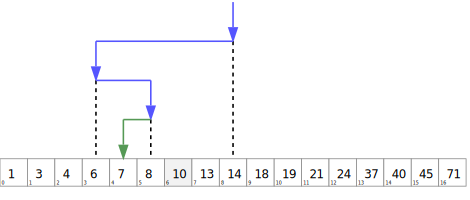
\includegraphics[width=0.7\linewidth]{img/Binary_Search_Depiction}
	\label{fig:binarysearchdepiction}
\end{figure}

Ahora supongamos que conocemos dos índices $L <R$ tal que $A_L \leq k \leq A_R$. Como la matriz está ordenada, podemos deducir que $k$ cualquiera de los dos ocurre entre $A_L, A_{L+1}, \dots, A_R$ o no aparece en la matriz en absoluto. Si elegimos un índice arbitrario $M$ tal que $L <M <R$ y comprobar si $k$ es menor o mayor que $A_M$. Tenemos dos casos posibles:

\begin{itemize}
	\item $A_L \leq k \leq A_M$. En este caso, reducimos el problema de $[L, R]$ a $[L,M]$.
	\item $A_M \leq k \leq A_R$. En este caso, reducimos el problema de $[L, R]$ a $[M,R]$.
\end{itemize}

Cuando es imposible elegir $M$, Eso es cuando $R = L + 1$, comparamos directamente $k$ con $A_L$ y $A_R$. De lo contrario, querríamos elegir $M$ de tal manera que reduzca el segmento activo a un solo elemento lo más rápidamente posible en el peor de los casos.

Dado que en el peor de los casos siempre reduciremos a un segmento mayor de $[L,M]$ y $[M,R]$. Así, en el peor de los casos la reducción sería de $R-L$ a $\max(M-L, R-M)$. Para minimizar este valor, debemos elegir $M \approx \frac{L+R}{2}$, entonces:

$$M-L \approx \frac{R-L}{2} \approx R-M.$$

En otras palabras, desde la perspectiva del peor de los casos, lo óptimo es elegir siempre $M$ en el medio de $[L, R]$ y dividirlo por la mitad. Por lo tanto, el segmento activo se reduce a la mitad en cada paso hasta que alcanza el tamaño $1$. Entonces, si el proceso necesita $h$ pasos, al final reduce la diferencia entre $R$ y $l$ de $R-L$ a $\frac{R-L}{2^h} \approx 1$, dándonos la ecuación $2^h \approx R-L$.

Tomando $\log_2$ en ambos lados, obtenemos $h \approx \log_2(R-L) \in O(\log n)$.

El número logarítmico de pasos es drásticamente mejor que el de la búsqueda lineal. Por ejemplo, para $n \approx 2^{20} \approx 10^6$ necesitarías realizar aproximadamente un millón de operaciones para la búsqueda lineal, pero solo alrededor $20$ operaciones con la búsqueda binaria.

\subsubsection{Límite inferior y límite superior}

A menudo es conveniente encontrar la posición del primer elemento que no sea menor que $k$ (llamado límite inferior de $k$ en la matriz) o la posición del primer elemento que es mayor que $k$ (llamado límite superior de $k$) en lugar de la posición exacta del elemento.

Juntos, los límites inferior y superior producen un medio intervalo posiblemente vacío de los elementos de la matriz que son iguales a $k$. Para comprobar si $k$ está presente en la matriz, es suficiente encontrar su límite inferior y verificar si el elemento correspondiente equivale a $k$.

La explicación anterior proporciona una descripción aproximada del algoritmo. Para los detalles de implementación, necesitaríamos ser más precisos.

Mantendremos un par $L <R$ tal que $A_L \leq k < A_R$. Lo que significa que el intervalo de búsqueda activa es $[L, R)$. Usamos medio intervalo aquí en lugar de un segmento. $[L, R]$ ya que resulta que requiere menos trabajo de caso.

Cuando $R = L+1$, podemos deducir de las definiciones anteriores que $R$ es el límite superior de $k$. Es conveniente inicializar $R$ con índice pasado el final, es decir $R=n$ y $l$ con índice antes del comienzo, es decir $L=-1$. Está bien siempre y cuando nunca evaluemos $A_L$ y $A_R$ en nuestro algoritmo directamente, tratándolo formalmente como $A_L = -\infty$ y $A_R = +\infty$.

Finalmente, para ser específico sobre el valor de $M$ elegimos, nos quedaremos con $M = \lfloor \frac{L+R}{2} \rfloor$.

\subsection{Buscar en predicado arbitrario}
Sea $f : \{0,1,\dots, n-1\} \to \{0, 1\}$  ser una función booleana definida en $f : \{0,1,\dots, n-1\} \to \{0, 1\}$  tal que aumenta monótonamente, es decir

$$ f(0) \leq f(1) \leq \dots \leq f(n-1). $$

La búsqueda binaria, como se describe arriba, encuentra la partición de la matriz por el predicado $f(M)$ , manteniendo el valor booleano de $k < A_M$  expresión. Es posible utilizar un predicado monótono arbitrario en lugar de $k < A_M$. Es particularmente útil cuando el cálculo de $f(k)$ esto requiere demasiado tiempo para calcularlo para cada valor posible. En otras palabras, la búsqueda binaria encuentra el índice único $L$ tal que $f(L) = 0$ y
$f(R)=f(L+1)=1$ si tal punto de transición existe, o nos da $L = n-1$ si $f(0) = \dots = f(n-1) = 0$ o $L = -1$  si $f(0) = \dots = f(n-1) = 1$.

Prueba de corrección suponiendo que exista un punto de transición, es decir $f(0)=0$ y $f(n-1)=1$: La implementación mantiene el bucle invariante $f(l)=0, f(r)=1$. . Cuando $r - l > 1$, la elección de $m$ medio $r-l$ siempre disminuirá. El bucle termina cuando $r - l = 1$, dándonos nuestro punto de transición deseado.

Esta situación ocurre a menudo cuando se nos pide que calculemos algún valor, pero solo somos capaces de verificar si este valor es al menos $i$. Por ejemplo, te dan una matriz $a_1,\dots,a_n$ y se le pide que encuentre la suma promedio máxima fijada

$$ \left \lfloor \frac{a_l + a_{l+1} + \dots + a_r}{r-l+1} \right\rfloor $$

entre todos los pares posibles de $l,r$ tal que $r-l \geq x$. Una de las formas sencillas de resolver este problema es comprobar si la respuesta es al menos $\lambda$ , eso si hay un par $l, r$  tal que lo siguiente es cierto:

$$ \frac{a_l + a_{l+1} + \dots + a_r}{r-l+1} \geq \lambda. $$

De manera equivalente, se reescribe como

$$ (a_l - \lambda) + (a_{l+1} - \lambda) + \dots + (a_r - \lambda) \geq 0, $$

entonces ahora necesitamos verificar si hay un subarreglo de un nuevo arreglo $a_i - \lambda$ de longitud al menos $x+1$ con suma no negativa, lo cual es factible con algunas sumas de prefijo.

\subsection{Búsqueda continua}
Dejar $f : \mathbf{R}  \to \mathbf{R} $ ser una función de valor real que es continua en un segmento $[L, R]$.

Sin pérdida de generalidad supongamos que $f(L) \leq f(R)$. Del teorema del valor intermedio se deduce que para cualquier $y \in [f(L), f(R)]$ hay $x \in [L, R]$ tal que $f(x) = y$. Tenga en cuenta que, a diferencia de los párrafos anteriores, no es necesario que la función sea monótona.

El valor $x$ podría aproximarse hasta $\pm\delta$ en $O\left(\log \frac{RL}{\delta}\right)$ tiempo para 
cualquier valor específico de $\delta$. La idea es esencialmente la misma, si tomamos $M \in (L, R)$ entonces 
podríamos reducir el intervalo de búsqueda a cualquiera de los dos $[L,M]$ o $[M,R]$ dependiendo de si $f(M)$ es mas grande que $y$ . Un ejemplo común aquí sería encontrar raíces de polinomios de grados impares.


Por ejemplo, dejemos $f(x)=x^3 + ax^2 + bx + c$. Entonces $f(L) \to -\infty$ y $f(R) \to +\infty$ con
$L \to -\infty$ y $R \to +\infty$. Lo que significa que siempre es posible encontrar cantidades 
suficientemente pequeñas $l$ y suficientemente grande $R$ tal que $f(L) < 0$ y $f(R) > 0$. Entonces, es 
posible encontrar con búsqueda binaria un intervalo arbitrariamente pequeño que contenga $x$ tal que $f(x)=0$ .

\subsection{Buscar con potencias de 2}
Otra forma notable de realizar una búsqueda binaria es, en lugar de mantener un segmento activo, mantener el puntero actual $i$ y la potencia actual $k$. El puntero comienza en $i=L$ y luego en cada iteración se prueba el predicado en el punto $i+2^k$. Si el predicado sigue siendo $0$, el puntero avanza desde $i$ a $i+2^k$, de lo contrario permanece igual, entonces el poder $k$ se reduce en $1$.

Este paradigma se usa ampliamente en tareas relacionadas con árboles, como encontrar el ancestro común más bajo de dos vértices o encontrar un ancestro de un vértice específico que tenga una altura determinada. También podría adaptarse para, por ejemplo, encontrar el $k$-ésimo elemento distinto de cero en un árbol de Fenwick.

%Trataremos de aprovechar el hecho de que la colección está ordenada y vamos a hacer algo distinto: nuestro espacio de búsqueda se irá achicando a segmentos cada vez menores de la colección original. La idea es descartar segmentos de la lista donde el valor seguro que no puede estar:

%\begin{enumerate}
%	\item Consideramos como segmento inicial de búsqueda a la lista completa.
%	\item Analizamos el punto medio del segmento (el valor central), si es el valor buscado, devolvemos el índice del punto medio.
%	\item Si el valor central es mayor al buscado, podemos descartar el segmento que está desde el punto medio hacia la a derecha.
%	\item Si el valor central es menor al buscado, podemos descartar el segmento que está desde el punto medio hacia la izquierda.
%	\item Una vez descartado el segmento que no nos interesa, volvemos a analizar el segmento restante, de la misma forma.
%	\item Si en algún momento el segmento a analizar tiene longitud 0 o negativa significa que el valor buscado no se encuentra en la coleción.
%\end{enumerate}

%Este algoritmo es un gran ejemplo de una estrategia de dividir y conquistar. Dividir y conquistar 
%significa que dividimos el problema en partes más pequeñas, resolvemos dichas partes más pequeñas de 
%alguna manera y luego reensamblamos todo el problema para obtener el resultado. Cuando realizamos una 
%búsqueda binaria en una colección, primero verificamos el ítem central. Si el ítem que estamos 
%buscando es menor que el ítem central, podemos simplemente realizar una búsqueda binaria en la mitad 
%izquierda de la colección original. Del mismo modo, si el ítem es mayor, podemos realizar una 
%búsqueda binaria en la mitad derecha. 

%Para señalar la porción del segmento que se está analizando a cada paso, utilizaremos dos variables (izq y der) que contienen la posición de inicio y la posición de fin del segmento que se está considerando. De la misma manera usaremos la varible medio para contener la posición del punto medio del segmento.

%En el gráfico que se incluye a continuación, vemos qué pasa cuando se busca el valor 18 en la lista [1, 3, 5, 7, 9, 11, 13, 15, 17, 19, 21, 23].

% TODO: \usepackage{graphicx} required
%\begin{figure}[h!]
%	\centering
%	\includegraphics[width=0.7\linewidth]{img/f0801}


%\end{figure}

